

\mode<presentation>
{
  \usetheme{boxes}
  %\useoutertheme{infolines}
  % með efnisyfirliti: Szeged, Frankfurt 
  % án efnisyfirlits: Pittsburgh
  % áhugavert: CambridgeUS, Boadilla
  %\setbeamercovered{transparent} %gegnsætt
  \setbeamercovered{invisible}

\defbeamertemplate*{footline}{infolines theme}
{
  \leavevmode%
  \hbox{%
  \begin{beamercolorbox}[wd=.333333\paperwidth,ht=2.25ex,dp=1ex,center]{author in head/foot}%
  %  \usebeamerfont{author in head/foot}\insertshortauthor~~\beamer@ifempty{\insertshortinstitute}{}{(\insertshortinstitute)}
  \end{beamercolorbox}%
  \begin{beamercolorbox}[wd=.333333\paperwidth,ht=2.25ex,dp=1ex,center]{title in head/foot}%
   % \usebeamerfont{title in head/foot}\insertshorttitle
  \end{beamercolorbox}%
  \begin{beamercolorbox}[wd=.333333\paperwidth,ht=2.25ex,dp=1ex,right]{date in head/foot}%
    %\usebeamerfont{date in head/foot}\insertshortdate{}\hspace*{2em}
    \insertshortlecture.\insertframenumber{} / \insertshortlecture.\inserttotalframenumber\hspace*{2ex} 
  \end{beamercolorbox}}%
  \vskip0pt%
}
\resetcounteronoverlays{rtaskno} %Does not increase counter rtaskno on \pause in beamer


}


\usepackage[english,icelandic]{babel}
\usepackage[utf8]{inputenc}
\usepackage{t1enc}
\usepackage{graphicx}
\usepackage{amsmath}
\usepackage{amssymb}
\usepackage{mathrsfs}
\usepackage{verbatim}
\usepackage{esint}

% RAGNAR SIGURÐSSON
%\usepackage[T1]{fontenc} 
%\usepackage[icelandic]{babel}
\usepackage{latexsym,amssymb,amsmath}
%\usepackage[utf8]{inputenc}
%\usepackage{graphicx}
\usepackage{epstopdf}
\usepackage{verbatim}
\usepackage{array,tabularx,arydshln}
\setbeamertemplate{theorems}[numbered]


\newtheorem{setning}{Setning}
\newtheorem{hjalpar}{Hjálparsetning}
\theoremstyle{definition}
\newtheorem{rithattur}{Ritháttur}
\newtheorem{skilgreining}{Skilgreining}
\newtheorem{daemi}{Dæmi}
\newtheorem{ath}{Athugasemd}

\newcommand\Wider[2][3em]{%
\makebox[\linewidth][c]{%
  \begin{minipage}{\dimexpr\textwidth+#1\relax}
  \raggedright#2
  \end{minipage}%
  }%
}

%counter used for blocks
\newcounter{rtaskno}
\DeclareRobustCommand{\rtask}[1]{%
   \refstepcounter{rtaskno}%
   \kaflanr.\thertaskno\label{#1}}

\newcommand{\C}{{\mathbb  C}}
\newcommand{\Z}{{\mathbb Z}}
\newcommand{\R}{{\mathbb  R}}
\newcommand{\N}{{\mathbb  N}}
\newcommand{\Q}{{\mathbb Q}}
\renewcommand{\phi}{\varphi}
\renewcommand{\epsilon}{\varepsilon}
\newcommand{\p}{{\partial}}
\renewcommand{\d}{{\partial}}

% RAGNAR SIGURÐSSON
\newcommand{\nin}{\mbox{$\;\not\in\;$}}
\newcommand{\dive}{\mbox{${\rm\bf div\,}$}}
\newcommand{\curl}{\mbox{${\rm\bf curl\,}$}}
\newcommand{\grad}{\mbox{${\rm\bf grad\,}$}}
\newcommand{\spann}{\mbox{${\rm Span}$}}
\newcommand{\tr}{\mbox{${\rm tr}$}}
\newcommand{\rank}{\mbox{${\rm rank}$}}
\newcommand{\image}{\mbox{${\rm image}$}}
\newcommand{\nullity}{\mbox{${\rm null}$}}
\newcommand{\proj}{\mbox{${\rm proj}$}}
\newcommand{\id}{\mbox{${\rm id}$}}
%\newcommand{\R}{\mbox{${\bf R}$}}
%\newcommand{\C}{\mbox{${\bf C}$}}
\newcommand{\Rn}{\mbox{${\bf R}^n$}}
\newcommand{\Rm}{\mbox{${\bf R}^m$}}
\newcommand{\Rk}{\mbox{${\bf R}^k$}}
\newcommand{\Av}{\mbox{${\bf A}$}}
\newcommand{\av}{\mbox{${\bf a}$}}
\newcommand{\uv}{\mbox{${\bf u}$}}
\newcommand{\vv}{\mbox{${\bf v}$}}
\newcommand{\wv}{\mbox{${\bf w}$}}
\newcommand{\xv}{\mbox{${\bf x}$}}
\newcommand{\zv}{\mbox{${\bf z}$}}
\newcommand{\yv}{\mbox{${\bf y}$}}
\newcommand{\bv}{\mbox{${\bf b}$}}
\newcommand{\cv}{\mbox{${\bf c}$}}
\newcommand{\dv}{\mbox{${\bf d}$}}
\newcommand{\ev}{\mbox{${\bf e}$}}
\newcommand{\fv}{\mbox{${\bf f}$}}
\newcommand{\gv}{\mbox{${\bf g}$}}
\newcommand{\hv}{\mbox{${\bf h}$}}
\newcommand{\iv}{\mbox{${\bf i}$}}
\newcommand{\jv}{\mbox{${\bf j}$}}
\newcommand{\kv}{\mbox{${\bf k}$}}
\newcommand{\pv}{\mbox{${\bf p}$}}
\newcommand{\nv}{\mbox{${\bf n}$}}
\newcommand{\qv}{\mbox{${\bf q}$}}
\newcommand{\rv}{\mbox{${\bf r}$}}
\newcommand{\sv}{\mbox{${\bf s}$}}
\newcommand{\tv}{\mbox{${\bf t}$}}
\newcommand{\ov}{\mbox{${\bf 0}$}}
\newcommand{\Fv}{\mbox{${\bf F}$}}
\newcommand{\Gv}{\mbox{${\bf G}$}}
\newcommand{\Uv}{\mbox{${\bf U}$}}
\newcommand{\Nv}{\mbox{${\bf N}$}}
\newcommand{\Hv}{\mbox{${\bf H}$}}
\newcommand{\Ev}{\mbox{${\bf E}$}}
\newcommand{\Sv}{\mbox{${\bf S}$}}
\newcommand{\Tv}{\mbox{${\bf T}$}}
\newcommand{\Bv}{\mbox{${\bf B}$}}
\newcommand{\Oa}{\mbox{$(0,0)$}}
\newcommand{\Ob}{\mbox{$(0,0,0)$}}
\newcommand{\Onv}{\mbox{$[0,0,\ldots,0]$}}
\newcommand{\an}{\mbox{$(a_1,a_2, \ldots,a_n)$}}
\newcommand{\xn}{\mbox{$(x_1,x_2, \ldots,x_n)$}}
\newcommand{\xnv}{\mbox{$[x_1,x_2, \ldots,x_n]$}}
\newcommand{\vnv}{\mbox{$[v_1,v_2, \ldots,v_n]$}}
\newcommand{\wnv}{\mbox{$[w_1,w_2, \ldots,w_n]$}}
\newcommand{\tvint}{\int\!\!\!\int}
\newcommand{\thrint}{\int\!\!\!\int\!\!\!\int}
\renewcommand{\ast}{{\operatorname{\text{astand}}}}


\usepackage{caption}
%\usepackage{pgfpages}
% \pgfpagesuselayout{2 on 1}[a4paper,border shrink=5mm]

\def\lecturename{Stærðfræðigreining IIB}
\title{\insertlecture}
\author{Sigurður Örn Stefánsson, \href{mailto:sigurdur@hi.is}{sigurdur@hi.is}}
\institute
{
  Verkfræði- og náttúruvísindasvið\\
  Háskóli Íslands
}
\subtitle{Stærðfræðigreining IIB, STÆ205G}
%\subject{\lecturename}

\mode<article>
{
	\usepackage[colorlinks=false,
	pdfauthor={Sigurður Örn Stefánson},
	%pdftitle={Töluleg greining}
	]{hyperref}
  %\usepackage{times}
  %\usepackage{mathptmx}
  \usepackage[left=1.5cm,right=4cm,top=1.5cm,bottom=3cm]{geometry}
}

% Beamer version theme settings

%\useoutertheme[height=0pt,width=2cm,right]{sidebar}
%\usecolortheme{rose,sidebartab}
%\useinnertheme{circles}
%\usefonttheme[only large]{structurebold}


\setbeamercolor{sidebar right}{bg=black!15}
\setbeamercolor{structure}{fg=blue}
\setbeamercolor{author}{parent=structure}

\setbeamerfont{title}{series=\normalfont,size=\LARGE}
\setbeamerfont{title in sidebar}{series=\bfseries}
\setbeamerfont{author in sidebar}{series=\bfseries}
\setbeamerfont*{item}{series=}
\setbeamerfont{frametitle}{size=}
\setbeamerfont{block title}{size=\small}
\setbeamerfont{subtitle}{size=\normalsize,series=\normalfont}


\setbeamertemplate{sidebar right}
{
  {\usebeamerfont{title in sidebar}%
    \vskip1.5em%
    \hskip3pt%
    \usebeamercolor[fg]{title in sidebar}%
    \insertshorttitle[width=2cm-6pt,center,respectlinebreaks]\par%
    \vskip1.25em%
  }%
  {%
    \hskip3pt%
    \usebeamercolor[fg]{author in sidebar}%
    \usebeamerfont{author in sidebar}%
    \insertshortauthor[width=2cm-2pt,center,respectlinebreaks]\par%
    \vskip1.25em%
  }%
  \hbox to2cm{\hss\insertlogo\hss}
  \vskip1.25em%
  \insertverticalnavigation{2cm}%
  \vfill
  \hbox to 2cm{\hfill\usebeamerfont{subsection in
      sidebar}\strut\usebeamercolor[fg]{subsection in
      sidebar}\insertshortlecture.\insertframenumber\hskip5pt}%
  \vskip3pt%
}%

\setbeamertemplate{title page}
{
  \vbox{}
  \vskip1em
  %{\huge Kapitel \insertshortlecture\par}
  {\usebeamercolor[fg]{title}\usebeamerfont{title}\inserttitle\par}%
  \ifx\insertsubtitle\@empty%
  \else%
    \vskip0.25em%
    {\usebeamerfont{subtitle}\usebeamercolor[fg]{subtitle}\insertsubtitle\par}%
  \fi%     
  \vskip1em\par
  %Vorlesung \emph{\lecturename}\ vom 
  \insertdate\par
  \vskip0pt plus1filll
  \leftskip=0pt plus1fill\insertauthor\par
  \insertinstitute\vskip1em
}

%\logo{\includegraphics[width=2cm]{beamerexample-lecture-logo.pdf}}



% Article version layout settings

\mode<article>

\makeatletter
\def\@listI{\leftmargin\leftmargini
  \parsep 0pt
  \topsep 5\p@   \@plus3\p@ \@minus5\p@
  \itemsep0pt}
\let\@listi=\@listI


\setbeamertemplate{frametitle}{\paragraph*{\insertframetitle\
    \ \small\insertframesubtitle}\ \par
}
\setbeamertemplate{frame end}{%
  \marginpar{\scriptsize\hbox to 1cm{\sffamily%
      \hfill\strut\insertshortlecture.\insertframenumber}\hrule height .2pt}}
\setlength{\marginparwidth}{1cm}
\setlength{\marginparsep}{1.5cm}

\def\@maketitle{\makechapter}

\def\makechapter{
  \newpage
  \null
  \vskip 2em%
  {%
    \parindent=0pt
    \raggedright
    \sffamily
    \vskip8pt
    %{\fontsize{36pt}{36pt}\selectfont Kapitel \insertshortlecture \par\vskip2pt}
    {\fontsize{24pt}{28pt}\selectfont \color{blue!50!black} \insertlecture\par\vskip4pt}
    {\Large\selectfont \color{blue!50!black} \insertsubtitle, \@date\par}
    \vskip10pt

    \normalsize\selectfont \@author\par\vskip1.5em
    %\hfill BLABLA
  }
  \par
  \vskip 1.5em%
}

\let\origstartsection=\@startsection
\def\@startsection#1#2#3#4#5#6{%
  \origstartsection{#1}{#2}{#3}{#4}{#5}{#6\normalfont\sffamily\color{blue!50!black}\selectfont}}

\makeatother

\mode
<all>



% Typesetting Listings

\usepackage{listings}
\lstset{language=Java}

\alt<presentation>
{\lstset{%
  basicstyle=\footnotesize\ttfamily,
  commentstyle=\slshape\color{green!50!black},
  keywordstyle=\bfseries\color{blue!50!black},
  identifierstyle=\color{blue},
  stringstyle=\color{orange},
  escapechar=\#,
  emphstyle=\color{red}}
}
{
  \lstset{%
    basicstyle=\ttfamily,
    keywordstyle=\bfseries,
    commentstyle=\itshape,
    escapechar=\#,
    emphstyle=\bfseries\color{red}
  }
}



% Common theorem-like environments

\theoremstyle{definition}
\newtheorem{exercise}[theorem]{\translate{Exercise}}




% New useful definitions:

\newbox\mytempbox
\newdimen\mytempdimen

\newcommand\includegraphicscopyright[3][]{%
  \leavevmode\vbox{\vskip3pt\raggedright\setbox\mytempbox=\hbox{\includegraphics[#1]{#2}}%
    \mytempdimen=\wd\mytempbox\box\mytempbox\par\vskip1pt%
    \fontsize{3}{3.5}\selectfont{\color{black!25}{\vbox{\hsize=\mytempdimen#3}}}\vskip3pt%
}}

\newenvironment{colortabular}[1]{\medskip\rowcolors[]{1}{blue!20}{blue!10}\tabular{#1}\rowcolor{blue!40}}{\endtabular\medskip}

\def\equad{\leavevmode\hbox{}\quad}

\newenvironment{greencolortabular}[1]
{\medskip\rowcolors[]{1}{green!50!black!20}{green!50!black!10}%
  \tabular{#1}\rowcolor{green!50!black!40}}%
{\endtabular\medskip}



\begin{document}

\section{Hlutafleiður}


\subsection{Graf falls} 

\subsubsection{Skilgreining }
Látum $f:\R^2\rightarrow \R$ vera fall.  {\em Graf} fallsins er skilgreint sem mengið 
$$\{(x,y,f(x,y))\mid (x,y)\in\R^2\}\subseteq \R^3.$$

Ef $f:\R^3\rightarrow \R$ er fall, þá er  {\em graf} fallsins skilgreint sem mengið 
$$\{(x,y,z,f(x,y,z))\mid (x,y,z)\in\R^3\}\subseteq \R^4.$$

            
 Dæmi: $f(x,y) = \sqrt{1-x^2-y^2}$, $-0.5\leq x,y\leq 0.5$.         

\begin{figure}[h]
\begin{center}
%\scalebox{0.45 }
\includegraphics{surface.png}
\caption*{ } 
\end{center}
\end{figure}  



\subsection{Jafnhæðarlínur}
 \subsubsection {Skilgreining }
  Látum $f:\R^2\rightarrow \R$ vera fall.  Ef $c$ er fasti þá er mengið 
$$\{(x,y)\mid f(x,y)=c\}\subseteq \R^2$$
kallað {\em jafnhæðarlína} eða {\em jafnhæðarferill} (e.~level curve) fallsins $f$ fyrir fastann $c$.

 Látum $f:\R^3\rightarrow \R$ vera fall.  Ef $c$ er fasti þá er mengið 
$$\{(x,y,z)\mid f(x,y,z)=c\}$$
kallað {\em jafnhæðarflötur} (e.~level surface)  
fallsins $f$ fyrir fastann $c$.
 


 Dæmi: $f(x,y) = \sqrt{1-x^2-y^2}$, $-0.5\leq x,y\leq 0.5$.         

\begin{figure}[h]
\begin{center} 
%\scalebox{0.45 }
\includegraphics{contour.png} 
\caption*{ }
\end{center}
\end{figure}  


\subsection{Fjarlægð milli punkta}
\subsubsection{Skilgreining }
 {\em Fjarlægðin} milli tveggja punkta 
$\xv=(x_1,x_2, \ldots,x_n)$ og $\yv=(y_1,y_2, \ldots,y_n)$ í $\Rn$ er skilgreind sem talan
$$|\xv-\yv|=\sqrt{(x_1-y_1)^2+(x_2-y_2)^2+\cdots+(x_n-y_n)^2}.$$
 



\subsection{Opnar kúlur}
 \subsubsection{Skilgreining }
  Látum $P=(p_1,p_2,\ldots,p_n)$ vera punkt í
$\Rn$.  Skilgreinum {\em opnu kúluna} með miðju í $P$ og geisla $r$ sem
mengið  
$$B_r(P)=\{Q\in\Rn\mid |Q-P|<r\}.$$
Í $\R^2$ er eðlilegra að tala um {\em opna skífu} eða {\em opinn disk} í stað opinnar kúlu og í $\R$ þá er talað um opin bil.  

 




\subsection{Opin mengi}
 \subsubsection{Skilgreining }
Látum $U$ vera hlutmengi í $\Rn$.

Sagt er að $U$ sé {\em opið mengi} ef um sérhvern punkt $P$ í $U$ gildir að til er tala $r>0$ þannig að $B_r(P)\subseteq U$.

Mengið $U$ er sagt {\em lokað} ef fyllimengið er opið.  ({\em Fyllimengi} $U$ er skilgreint sem mengið 
$\Rn\setminus U=\{Q\in \Rn\mid Q\nin U\}$.)




\subsection{Jaðarpunktur}
 \subsubsection{Skilgreining }
Látum $U$ vera mengi í $\Rn$.  Punktur $P$ í $\Rn$ er sagður {\em jaðarpunktur} $U$ ef sérhver opin kúla $B_r(P)$ með $r>0$ inniheldur bæði punkt úr $U$ og punkt úr $\Rn\setminus U$.   (Athugið að bæði er mögulegt að jaðarpunktur $U$ sé í $U$ og að hann sé ekki í $U$.)



\subsection{Skilgreiningarmengi}
 \subsubsection{Skilgreining }
Fyrir fall $f(x_1,x_2,\ldots,x_n)$ þá táknar ${\cal D}(f)$ skilgreiningarmengi fallsins $f$.
Ef fallið er gefið með formúlu og ekkert sagt um ${\cal D}(f)$ þá lítum við svo á að ${\cal D}(f)$ sé mengi allra punkta í $\Rn$ þannig að formúlan gefi vel skilgreinda tölu.




\subsection{Markgildi}
 \subsubsection{Skilgreining }
Látum $f(x_1,x_2,\ldots,x_n)$ vera fall af
$n$ breytistærðum með skilgreiningarmengi ${\cal D}(f)\subseteq \Rn$.
Látum $P=(p_1,p_2,\ldots,p_n)$ vera punkt í $\Rn$ þannig að sérhver
opin kúla um $P$ inniheldur meira en einn punkt úr ${\cal D}(f)$. 

\smallskip 
\noindent
Segjum að $f(x_1,x_2,\ldots,x_n)$  stefni á tölu $L$ þegar
$(x_1,x_2,\ldots,x_n)$  stefnir á $(p_1,p_2,\ldots,p_n)$ ef
eftirfarandi gildir: 

\smallskip
\noindent
{\em Fyrir sérhverja tölu $\epsilon>0$ er til tala $\delta>0$
þannig að ef $(x_1,x_2,\ldots,x_n)\in{\cal D}(f)$ og  
$$|(x_1,x_2,\ldots,x_n)-(p_1,p_2,\ldots,p_n)|<\delta$$ 
þá er 
$$|f(x_1,x_2,\ldots,x_n)-L|<\epsilon.$$}


\subsubsection{Ritháttur }
Ef $f(x_1,x_2,\ldots,x_n)$  stefnir á tölu $L$ þegar $(x_1,x_2,\ldots,x_n)$  stefnir á $(p_1,p_2,\ldots,p_n)$ þá er ritað 
$$\lim_{(x_1,x_2,\ldots,x_n)\rightarrow (p_1,p_2,\ldots,p_n)}
f(x_1,x_2,\ldots,x_n)=L.$$
 

 \subsubsection{Skilgreining  (Skilgreining 4.8 sett fram fyrir föll af tveimur breytum.)  }
 
  
Látum $f(x,y)$ vera fall skilgreint á mengi  ${\cal D}(f)\subseteq \R^2$.  Látum $(a,b)$ vera punkt í $\R^2$ þannig að sérhver opin skífa um $(a,b)$ inniheldur meira en einn punkt úr ${\cal D}(f)$.

Segjum að $f(x,y)$  stefni á tölu $L$ þegar $(x,y)$  stefnir á $(a,b)$ ef eftirfarandi gildir:

\smallskip
\noindent
{\em fyrir sérhverja tölu $\epsilon>0$ er til tala $\delta>0$
þannig að ef $(x,y)\in{\cal D}(f)$ og
$$\delta>|(x,y)-(a,b)|=\sqrt{(x-a)^2+(y-b)^2}$$ 
þá er  
$$|f(x,y)-L|<\epsilon.$$}

 




\subsection{Reglur um markgildi}
 \subsubsection{Setning }
  Látum $f$ og $g$ vera föll af tveimur breytum.  Gerum ráð  fyrir að 
$$\lim_{(x,y)\rightarrow (a,b)}f(x,y)=L\quad\mbox{og}\quad
\lim_{(x,y)\rightarrow (a,b)}g(x,y)=M,$$
og að sérhver grennd um $(a,b)$ innihaldi fleiri en einn punkt þar sem bæði föllin $f$ og $g$ eru skilgreind. Þá gildir

{\bf (a)}  $\lim_{(x,y)\rightarrow (a,b)}(f(x,y)\pm g(x,y))=L\pm M$.

{\bf (b)}  $\lim_{(x,y)\rightarrow (a,b)}f(x,y) g(x,y)=LM$.

{\bf (c)}  $\lim_{(x,y)\rightarrow (a,b)}\frac{f(x,y)}{g(x,y)}=
\frac{L}{M}$, svo framarlega sem $M\neq 0$.

{\bf (d)}  $\lim_{(x,y)\rightarrow (a,b)}F(f(x,y))=F(L)$ ef $F$ er fall af einni breytistærð sem er samfellt í punktinum $L$.
 
 




\subsection{Samfelldni}
 \subsubsection{Skilgreining }
   Látum $f$ vera fall af $n$ breytistærðum skilgreint á mengi ${\cal D}(f)$ í $\Rn$.  Fallið $f$ er sagt {\em samfellt í punkti} 
$(p_1,p_2,\ldots,p_n)$ í ${\cal D}(f)$
ef 
$$\lim_{(x_1,x_2,\ldots,x_n)\rightarrow (p_1,p_2,\ldots,p_n)}
f(x_1,x_2,\ldots,x_n)=f(p_1,p_2,\ldots,p_n).$$

Sagt er að fallið sé {\em samfellt} ef það er samfellt í öllum punktum skilgreiningarmengis síns.

 


\subsection{Hlutafleiður}
\subsubsection{Skilgreining }
 Látum $f(x,y)$ vera fall af tveimur breytum $x$ og $y$ sem er skilgreint á opinni skífu með miðju í punktinum $(a,b)$. 
 
 \medskip
 Skilgreinum \emph{hlutafleiðu m.t.t.} $x$ í $(a,b)$ með
$$f_1(a,b)=\lim_{h\rightarrow 0}\frac{f(a+h,b)-f(a,b)}{h}$$
og \emph{hlutafleiðu m.t.t.} $y$ í $(a,b)$ með
$$f_2(a,b)=\lim_{k\rightarrow 0}\frac{f(a,b+k)-f(a,b)}{k}$$

ef markgildin eru til.


 \begin{figure}[!h]
        \centering
        \begin{minipage}{\textwidth}
            \centering
            \includegraphics[width=1\linewidth]{xpart.png}
            \caption*{Hlutafleiða m.t.t.~$x$ fyrir $y=1$.}
        \end{minipage}%
        \begin{minipage}{\textwidth}
            \centering
            \includegraphics[width=1\linewidth]{ypart.png}
            \caption*{Hlutafleiða m.t.t.~$y$ fyrir $x=1$.}
        \end{minipage}
   \end{figure}
 


\subsubsection{Skilgreining }
  
Látum $f(x,y,z)$ vera fall af þremur breytum $x$, $y$ og $z$ sem er skilgreint á opinni kúlu með miðju í punktinum $(a, b,c)$. 

\medskip

Skilgreinum \emph{hlutafleiðu m.t.t.} $x$ í $(a,b,c)$ með
$$f_1(a,b,c)=\lim_{h\rightarrow 0}\frac{f(a+h,b,c)-f(a,b,c)}{h},$$
 \emph{hlutafleiðu m.t.t.} $y$ í $(a,b,c)$ með
$$f_2(a,b,c)=\lim_{k\rightarrow 0}\frac{f(a,b+k,c)-f(a,b,c)}{k}$$

og \emph{hlutafleiðu m.t.t.} $z$ í $(a,b,c)$ með
$$f_3(a,b,c)=\lim_{\ell\rightarrow 0}\frac{f(a,b,c+\ell)-f(a,b,c)}{\ell}$$

ef markgildin eru til.
 


\subsubsection{Skilgreining }
Látum $f$ vera fall af
$n$ breytum $x_1,x_2,\ldots,x_n$ sem er skilgreint á opinni kúlu um punktinn $\mathbf{a}=(a_1, a_2, \ldots, a_n).$ 

\medskip	
{\em Hlutafleiða} $f$ með
tilliti til breytunnar $x_k$ í punktinum $\mathbf{a}$ er skilgreind sem markgildið 
$$f_k(\mathbf{a})=\lim_{h\rightarrow 0}\frac{f(\mathbf{a}+h\ev_k)-f(\mathbf{a})}{h}$$
ef markgildið er til.  (Hér stendur $\ev_k$ fyrir vigurinn sem er með
0 í öllum hnitum nema því $k$-ta þar sem er 1.)


\Wider{\subsubsection{Ritháttur }
   Ritum $z=f(x,y)$.  Ýmis konar ritháttur fyrir hlutafleiður, m.a.~
$$f_1(x,y)=\frac{\partial z}{\partial x}=  \frac{\partial }{\partial x}f(x,y)
=D_1f(x,y)=f_x(x,y)=D_xf(x,y)=\partial_xf(x,y)$$

$$f_2(x,y)=\frac{\partial z}{\partial y}=  \frac{\partial }{\partial y}f(x,y)
=D_2f(x,y)=f_y(x,y)=D_yf(x,y)=\partial_yf(x,y)$$

Þegar við viljum tákna gildið á hlutafleiðu $f$ í ákveðnum punkti
$(x,y)=(a,b)$ þá eru líka ýmsir möguleikar, til dæmis 
$$\frac{\partial z}{\partial x}\bigg|_{(a,b)}=
\left(\frac{\partial }{\partial x}f(x,y)\right)\bigg|_{(a,b)}
=f_1(a,b)=D_1f(a,b)$$
 $$\frac{\partial z}{\partial y}\bigg|_{(a,b)}=
\left(\frac{\partial }{\partial y}f(x,y)\right)\bigg|_{(a,b)}
=f_2(a,b)=D_2f(a,b).$$
 }



\subsection{Snertiplan}
  Látum $f(x,y)$ vera fall af tveimur breytistærðum þannig að hlutafleiðurnar $f_1(a,b)$ og $f_2(a,b)$ séu skilgreindar.
  \begin{figure}
           \centering
            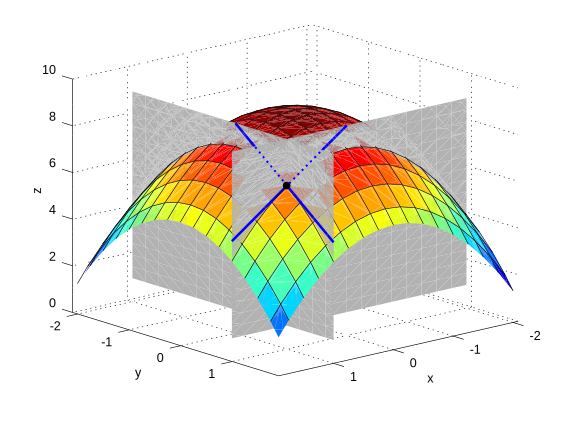
\includegraphics[width=0.6\linewidth]{bothpart.png}
	\caption*{}
    \end{figure}
    Í punktinum $(a,b,f(a,b))$ er 
    
    $\Tv_1 = \iv + f_1(a,b)\kv\qquad$ snertivigur við ferilinn $f(x,b) = z$ og
    
    $\Tv_2 = \jv + f_2(a,b)\kv\qquad$ snertivigur við ferilinn $f(a,y) = z$.



 Táknum með $S$ planið sem hefur stikunina
$$(a,b,f(a,b))+s\Tv_1+t\Tv_2, \quad -\infty < s,t < \infty.$$
Vigurinn 
$$\nv=\Tv_2\times \Tv_1=f_1(a,b)\iv+f_2(a,b)\jv-\kv$$ 

er þvervigur á $S$ og jafna plansins $S$ er
$$z=f(a,b)+f_1(a,b)(x-a)+f_2(a,b)(y-b).$$

\emph{Þverlína} á $S$ hefur stikun
$$(a,b,f(a,b)) + u \nv, \quad -\infty < u < \infty.$$

Ef $f(x,y)$ er 'nógu nálægt' (skilgreint nánar síðar) planinu $S$ þegar $(x,y)$ er nálægt punktinum $(a,b)$ þá kallast $S$ \emph{snertiplan} við grafið $z=f(x,y)$ í punktinum $(a,b,f(a,b)$.


\subsection{Hlutafleiður af hærra stigi}
 \subsubsection{Skilgreining }
  Ritum $z=f(x,y)$.  {\em Annars stigs
  hlutafleiður} $f$ eru skilgreindar með formúlunum
$$\frac{\partial^2 z}{\partial x^2}=
\frac{\partial}{\partial x} \frac{\partial z}{\partial x}
=f_{11}(x,y)=f_{xx}(x,y),$$
$$\frac{\partial^2 z}{\partial y^2}=
\frac{\partial}{\partial y} \frac{\partial z}{\partial y}
=f_{22}(x,y)=f_{yy}(x,y),$$
$$\frac{\partial^2 z}{\partial x\partial y}=
\frac{\partial}{\partial x} \frac{\partial z}{\partial y}
=f_{21}(x,y)=f_{yx}(x,y),$$
$$\frac{\partial^2 z}{\partial y\partial x}=
\frac{\partial}{\partial y} \frac{\partial z}{\partial x}
=f_{12}(x,y)=f_{xy}(x,y).$$

Hlutafleiðurnar $f_{11}(x,y)$ og $f_{22}(x,y)$ kallast hreinar
hlutafleiður og $f_{12}(x,y)$ og $f_{21}(x,y)$ kallast blandaðar
hlutafleiður.  
 

 \subsubsection{Setning }
  Látum $f(x,y)$ vera fall sem er skilgreint á opinni
skífu $D$ með miðju í $P=(a,b)$ .  Gerum ráð fyrir að
hlutafleiðurnar $f_1(x,y)$, $f_2(x,y)$, $f_{12}(x,y)$ og $f_{21}(x,y)$
séu allar skilgreindar á $D$ og að þær séu allar samfelldar á $D$.  Þá
gildir að 
$$f_{12}(a,b)=f_{21}(a,b).$$
 


 \subsubsection{Hugmynd að skilgreiningu }
  Skilgreiningu~5.6 má útvíkka á augljósan hátt
til að skilgreina 2.~stigs hlutafleiður fyrir föll af fleiri en
tveimur breytum.   Einnig er augljóst hvernig má skilgreina
hlutafleiður af hærri stigum en 2, til dæmis ef $w=f(x,y,z)$ þá 
$$\frac{\partial^3 w}{\partial x\partial y^2} \quad\quad\mbox{(diffra
    fyrst tvisvar m.t.t. }y\mbox{, svo einu sinni m.t.t. } x\mbox{)}$$
og 
$$\frac{\partial^3 w}{\partial y\partial z\partial y} \quad\quad\mbox{(diffra
    fyrst m.t.t. } y\mbox{, svo m.t.t. } z
\mbox{ og að lokum m.t.t. }y\mbox{)}.$$

 
 \subsubsection{Setning  (Almenn útgáfa af Setningu~5.7)}
     Látum $f$ vera
fall $n$ breytistærðum sem er skilgreint á opinni kúlu með miðju í 
$P=(x_1, x_2,\ldots, x_n)$.  

\medskip
Skoðum tvær hlutafleiður $f$ í punktum $P$
þar sem er diffrað með tilliti til sömu breytistærða og jafn oft með
tilliti til hverrar breytistærðar.  Ef þessar hlutafleiður eru
samfelldar í punktinum $P$ og allar hlutafleiður af lægra stigi eru
skilgreindar á $D$ og samfelldar á $D$ þá eru hlutafleiðurnar sem við
erum að skoða jafnar í $P$.
 

 \subsubsection {Dæmi:} 
 Ef $w = f(x,y,z)$ er fall af þremur breytistærðum þá er t.d.~
 \begin {equation*}
  \frac{\partial^4 w}{\partial x^2\partial y \partial z} = \frac{\partial^4 w}{\partial x \partial y \partial x \partial z}
 \end {equation*}
ef skilyrðin í setningunni eru uppfyllt.
  
 


\subsection{Keðjuregla} 

\subsubsection{Setning  (Keðjureglan í einni breytistærð.)}
 Gerum ráð fyrir að fallið $f(u)$ sé diffranlegt í punktinum $u=g(x)$ og að fallið $g(x)$ sé diffranlegt í punktinum $x$.  Þá er fallið $(f\circ g)(x)=f(g(x))$ diffranlegt í $x$ og 
$$(f\circ g)'(x)=f'(g(x))g'(x).$$


\subsubsection{Setning }
Látum $f(x,y)$ vera fall þar sem $x=x(t)$ og $y=y(t)$ eru föll af breytu $t$,  Gerum ráð fyrir að á opinni skífu um  punktinum $(x(t),y(t))$ séu báðar fyrsta stigs hlutafleiður $f$ skilgreindar og samfelldar.   Gerum enn fremur ráð fyrir að föllin $x(t)$ og $y(t)$ séu bæði diffranleg í punktinum $t$.  Þá er fallið 
$$g(t)=f(x(t),y(t))$$
diffranlegt í $t$ og 
$$g'(t)=f_1(x(t),y(t))x'(t)+f_2(x(t),y(t))y'(t).$$



\subsubsection{Ritháttur }

Ritum $z=f(x,y)$ þar sem $x=x(t)$ og $y=y(t)$ eru föll af breytu $t$.  Þá er 
$$\frac{dz}{dt}=\frac{\partial z}{\partial x}\frac{dx}{dt}
+\frac{\partial z}{\partial y}\frac{dy}{dt}.$$

 \begin{figure}[h!]
           \centering
            \includegraphics[width=0.3\linewidth]{chain1.png}
	\caption*{}
    \end{figure}


\subsubsection{Setning }
 Látum $f(x,y)$ vera fall af breytistærðum $x$ og $y$ sem aftur eru föll af breytum $s$ og $t$, það er að segja 
$x=x(s,t)$ og $y=y(s,t)$.  Ritum svo 
$$g(s,t)=f(x(s,t),y(s,t)).$$
Þá gildir (að gefnum sambærilegum skilyrðum og í 6.2) að
$$g_1(s,t)=f_1(x(s,t),y(s,t))x_1(s,t)+f_2(x(s,t),y(s,t))y_1(s,t),$$
og 
$$g_2(s,t)=f_1(x(s,t),y(s,t))x_2(s,t)+f_2(x(s,t),y(s,t))y_2(s,t).$$



\subsubsection{Ritháttur }

Ritum $z=f(x,y)$ þar sem $x=x(s,t)$ og $y=y(s,t)$ eru föll af breytum $s$ og  $t$.  Þá er 
$$\frac{\partial z}{\partial s}=
\frac{\partial z}{\partial x}\frac{\partial x}{\partial s}
+\frac{\partial z}{\partial y}\frac{\partial y}{\partial s}, \quad \text{og}\quad \frac{\partial z}{\partial t}=
\frac{\partial z}{\partial x}\frac{\partial x}{\partial t}
+\frac{\partial z}{\partial y}\frac{\partial y}{\partial t}.$$

 \begin{figure}[h!]
           \centering
            \includegraphics[width=0.35\linewidth]{chain2.png}
	\caption*{}
    \end{figure}


\subsubsection{Ritháttur}
 Ritum $z=f(x,y)$ þar sem $x=x(s,t)$ og $y=y(s,t)$ eru föll af breytum $s$ og  $t$.  Þá er 
$$\begin{bmatrix}\frac{\partial z}{\partial s} 
& \frac{\partial z}{\partial t}\end{bmatrix}
=\begin{bmatrix}\frac{\partial z}{\partial x} 
& \frac{\partial z}{\partial y}\end{bmatrix}
\begin{bmatrix}\frac{\partial x}{\partial s} 
& \frac{\partial x}{\partial t}\\
\frac{\partial y}{\partial s} 
& \frac{\partial y}{\partial t}
\end{bmatrix}$$

 

\subsubsection{Setning }
Látum $u$ vera fall af $n$ breytum $x_1, x_2, \ldots, x_n$ þannig að hvert $x_i$ má rita sem fall af $m$ breytum $t_1, t_2, \ldots, t_m$.  Gerum ráð fyrir að allar hlutafleiðurnar $\frac{\partial u}{\partial x_i}$ og $\frac{\partial x_i}{\partial t_j}$ séu til og samfelldar.  Þegar $u$ er skoðað sem fall af breytunum $t_1, t_2, \ldots, t_m$ fæst að 
$$\frac{\partial u}{\partial t_j}=
\frac{\partial u}{\partial x_1}\frac{\partial x_1}{\partial t_j}
+\frac{\partial u}{\partial x_2}\frac{\partial x_2}{\partial t_j}
+\cdots+
\frac{\partial u}{\partial x_n}\frac{\partial x_n}{\partial t_j}.$$

\begin{figure}[h!]
           \centering
            \includegraphics[width=0.45\linewidth]{chain3.png}
	\caption*{}
    \end{figure}


\subsubsection{Dæmi }
Látum $T$ vera fall af fall af $x$, $y$ og $t$, og $x$ og $y$ föll af $t$. Finnum $\frac{ dT}{dt}$.

\begin{figure}[h!]
           \centering
            \includegraphics[width=0.35\linewidth]{chain5.png}
	\caption*{}
    \end{figure}
$$\frac{d T}{d t} = \frac{\partial T}{\partial x} \frac{d x}{d t} +\frac{\partial T}{\partial y} \frac{d y}{\partial t} + \frac{\partial T}{\partial t} .$$


\subsubsection{Dæmi }
Látum $T$ vera fall af fall af $x$, $y$, $s$ og $t$, og $x$ og $y$ föll af $s$ og $t$. Finnum $\frac{ \partial T}{\partial t}$.

\begin{figure}[h!]
           \centering
            \includegraphics[width=0.45\linewidth]{chain6.png}
	\caption*{}
    \end{figure}
$$\frac{\partial T}{\partial t} = \frac{\partial T}{\partial x} \frac{\partial x}{\partial t} +\frac{\partial T}{\partial y} \frac{\partial y}{\partial t} + \left(\frac{\partial T}{\partial t}\right)_{x,y,s} .$$


\subsubsection{Dæmi }
Látum $z$ vera fall af fall af $u$, $v$ og $r$, $u$ og $v$ vera föll af $x$, $y$ og $r$ og $r$ vera fall af $x$ og $y$. Skrifum niður $\frac{\partial z}{\partial x}$.

\begin{figure}[h!]
           \centering
            \includegraphics[width=0.45\linewidth]{chain4.png}
	\caption*{}
    \end{figure}
$$\frac{\partial z}{\partial x} = \frac{\partial z}{\partial u} \frac{\partial u}{\partial x} +\frac{\partial z}{\partial u} \frac{\partial u}{\partial r} \frac{\partial r}{\partial x} 
+ \frac{\partial z}{\partial v} \frac{\partial v}{\partial x} + \frac{\partial z}{\partial v} \frac{\partial v}{\partial r} \frac{\partial r}{\partial x} +\frac{\partial z}{\partial r} \frac{\partial r}{\partial x}.$$




\subsection{Jákvætt einsleit föll} 

\subsubsection{Skilgreining }

Fall $f(x_1, x_2, \ldots, x_n)$ er sagt vera {\em jákvætt einsleitt af stigi} $k$ (e.~positively homogeneous of degree $k$) ef fyrir sérhvern punkt $(x_1, x_2, \ldots, x_n)$ og sérhverja tölu $t>0$ gildir að 
$$f(tx_1, tx_2, \ldots, tx_n)=t^kf(x_1, x_2, \ldots, x_n).$$


\subsubsection{Setning }
 Ef fall $f(x_1, x_2, \ldots, x_n)$ hefur samfelldar fyrsta stigs hlutafleiður og er jákvætt einsleitt af stigi $k$ þá er 
$$\sum_{i=1}^n x_if_i(x_1, x_2, \ldots, x_n)=kf(x_1, x_2, \ldots, x_n).$$ 
 



\subsection{Diffranleiki í einni breytistærð} 

\subsubsection{Skilgreining  }
  Látum $f$ vera fall af einni breytistærð og gerum ráð fyrir að $f$ sé
skilgreint á opnu bili sem inniheldur punktinn $a$.  Fallið $f$ er
sagt vera {\em diffranlegt} í punkti $a$ ef markgildið
$$f'(a)=\lim_{h\rightarrow 0}\frac{f(a+h)-f(a)}{h}$$
er til.



\subsection{Diffranleiki í einni breytistærð - önnur lýsing} 

\subsubsection{Skilgreining  }
Látum $f$ vera fall af einni breytistærð og gerum ráð fyrir að $f$ sé
skilgreint á opnu bili sem inniheldur punktinn $a$.  Fallið $f$ er
sagt vera {\em diffranlegt} í punkti $a$ ef til er tala $m$ þannig að
ef $L(x)=f(a)+m(x-a)$ þá er 
$$\lim_{h\rightarrow 0}\frac{f(a+h)-L(a+h)}{h}=0.$$
(Talan $m$ verður að vera jöfn $f'(a)$.)


\bigskip
Fallið $f$ er 'nálægt' línunni $L$ nálægt punktinum $a$.


\subsection{Diffranleiki} 

\subsubsection{Skilgreining }
Fall $f(x,y)$ sem er skilgreint á opinni
skífu umhverfis $(a,b)$ er sagt vera diffranlegt í punktinum $(a,b)$
ef báðar fyrsta stigs hlutafleiður $f$ eru skilgreindar í $(a,b)$ og ef 
$$\lim_{(h,k)\rightarrow (0,0)}
\frac{f(a+h, b+k)-S(a+h,b+k)}{\sqrt{h^2+k^2}}=0$$
þar sem $S(x,y) = f(a,b) + f_1(a,b)(x-a)+f_2(a,b)(y-b)$.

\bigskip
Fallið $f$ er 'nálægt' sléttunni $S$ nálægt punktinum $(a,b)$.


\subsection{Snertiplan}
  Ef $f$ er diffranlegt í $(a,b)$ þá kallast planið $S$ \emph{snertiplan} við graf fallsins.
  \begin{figure}
           \centering
            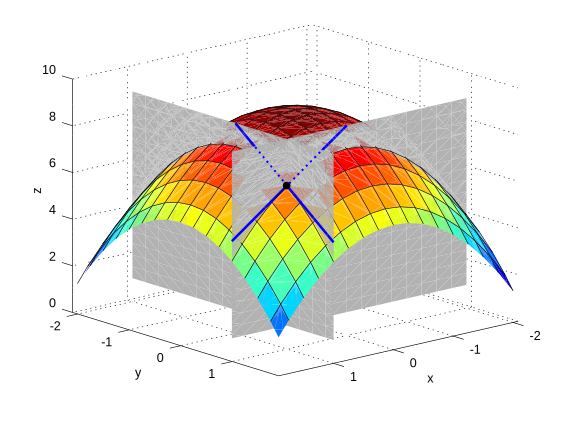
\includegraphics[width=0.6\linewidth]{bothpart.png}
	\caption*{}
    \end{figure}
    $S(x,y) = f(a,b) + f_1(a,b)(x-a)+f_2(a,b)(y-b)$.



\subsection{Diffranleiki} 

\subsubsection{Setning  (Meðalgildissetningin)}
Gerum ráð fyrir að fallið $f$
sé samfellt á lokaða bilinu $[a,b]$ og diffranlegt á opna bilinu
$(a,b)$.  Þá er til punktur $c$ á opna bilinu $(a,b)$ þannig að 
$$f(b)-f(a)=f'(c)(b-a).$$




\subsubsection{Setning }

Látum  $f(x,y)$ vera fall
sem er skilgreint á opinni 
skífu $\cal D$ með miðju í $(a,b)$ þannig að á þessari skífu eru báðar
fyrsta stigs hlutafleiður $f$ skilgreindar og samfelldar.  Gerum ráð fyrir að $h$
og $k$ séu tölur þannig að $(x+h, y+k)\in{\cal D}$.  Þá eru til tölur
$\theta_1$ og $\theta_2$ á milli 0 og 1 þannig að 
$$f(a+h,b+k)-f(a,b)=hf_1(a+\theta_1h,b+k)+kf_2(a,b+\theta_2k).$$


\subsubsection{Setning }
  Látum  $f(x,y)$ vera fall
sem er skilgreint á opinni 
skífu $\cal D$ með miðju í $(a,b)$ þannig að á þessari skífu eru báðar
fyrsta stigs hlutafleiður $f$ skilgreindar og samfelldar. 
Þá er fallið $f$ diffranlegt í $(a,b)$.




\subsubsection{Setning }
  Gerum ráð fyrir að $f(x,y)$ sé fall sem er
diffranlegt í punktinum $(a,b)$.  Þá er $f$ samfellt í $(a,b)$.




\subsubsection{Keðjuregla }
 Ritum $z=f(x,y)$ þar sem $x=x(s,t)$ og
$y=y(s,t)$.  Gerum ráð fyrir að 

\begin{enumerate}[(i)]
\item $x(a,b)=p$ og $y(a,b)=q$;
\item fyrsta stigs hlutafleiður $x(s,t)$ og $y(s,t)$ eru skilgreindar í
punktinum $(a,b)$;
\item fallið $f$ er diffranlegt í punktinum $(p,q)$.
\end{enumerate}

Þá eru fyrsta stigs hlutafleiður $z$ með tilliti til breytanna $s$ og
$t$ skilgreindar í punktinum $(a,b)$ og um þær gildir að 
$$\frac{\partial z}{\partial s}=
\frac{\partial z}{\partial x}\frac{\partial x}{\partial s}
+\frac{\partial z}{\partial y}\frac{\partial y}{\partial s}$$
og
$$\frac{\partial z}{\partial t}=
\frac{\partial z}{\partial x}\frac{\partial x}{\partial t}
+\frac{\partial z}{\partial y}\frac{\partial y}{\partial t}.$$




\subsection{Diffur} 

\subsubsection{Skilgreining }
  Ritum $z=f(x_1, x_2, \ldots, x_n)$.  {\em
  Diffrið} af $z$ er skilgreint sem 
$$dz=df=\frac{\partial z}{\partial x_1}dx_1
+\frac{\partial z}{\partial x_2}dx_2
+\cdots+\frac{\partial z}{\partial x_n}dx_n.$$
Diffrið er nálgun á 
$$\Delta f=f(x_1+dx_1, x_2+dx_2,\ldots,
x_n+dx_n)-f(x_1,x_2,\ldots,x_n).$$




\subsection{Varpanir $\Rn\rightarrow\Rm$} 
\subsubsection{Táknmál }
Látum $\fv:\Rn\rightarrow\Rm$ tákna vörpun.
Ritum $\fv=(f_1,\ldots,f_m)$ þar sem hvert $f_i$ er fall
$\Rn\rightarrow\R$.  Fyrir punkt í $\Rn$ ritum við
$\xv=(x_1,x_2,\ldots,x_n)$.  Síðan ritum við $\yv=\fv(\xv)$ þar sem 
$\yv=(y_1,y_2,\ldots,y_m)$ og 
\Wider{$$y_1=f_1(x_1,x_2,\ldots,x_n),y_2=f_2(x_1,x_2,\ldots,x_n),
\ldots, y_m=f_m(x_1,x_2,\ldots,x_n).$$}




\subsection{Jacobi-fylki} 
 \subsubsection{Skilgreining }
 Notum táknmálið úr 7.8.
Ef allar hlutafleiðurnar $\partial
y_i/\partial x_j$ eru skilgreindar í punktinum $\xv$ þá skilgreinum
við {\em Jacobi-fylki} $f$ í punktinum $\xv$ sem $m\times n$ fylkið
$$D\fv(\xv)=\begin{bmatrix}
\frac{\partial y_1}{\partial x_1}&\frac{\partial y_1}{\partial x_2}&
\cdots&\frac{\partial y_1}{\partial x_n}\\
\frac{\partial y_2}{\partial x_1}&\frac{\partial y_2}{\partial x_2}&
\cdots&\frac{\partial y_2}{\partial x_n}\\
\vdots&\vdots&\ddots&\vdots\\
\frac{\partial y_m}{\partial x_1}&\frac{\partial y_m}{\partial x_2}&
\cdots&\frac{\partial y_m}{\partial x_n}
\end{bmatrix}$$



\subsection{Diffranleiki varpana $\Rn\rightarrow\Rm$} 
 \subsubsection{Skilgreining }
 Notum táknmálið úr 7.8 og 7.9. Látum $\av=(a_1, a_2, \ldots, a_n)$ vera fastan punkt í $\Rn$ og ritum 
$\hv=(h_1,h_2,\ldots,h_n)$.  Vörpunin $\fv$ er
sögð diffranleg í punktinum $\av$ ef
$$\lim_{\hv\rightarrow
  \ov}\frac{|\fv(\av+\hv)-\fv(\av)-D\fv(\av)\hv|}{|\hv|}=0.$$ 

\bigskip
Vörpunin $f$ er 'nálægt' línulegu vörpuninni $D\fv$ nálægt punktinum $\av$.

\bigskip
Línulega vörpunin $D\fv$ kallast afleiða $\fv$.



\subsection{Keðjureglan} 
 \subsubsection{Setning }
Látum $\fv:\Rn\rightarrow \Rm$ og 
$\gv:\Rm\rightarrow \Rk$ vera varpanir.  Gerum ráð fyrir að vörpunin
$\fv$ sé diffranleg í punkti $\xv$ og vörpunin $\gv$ sé diffranleg í
punktinum $\yv=\fv(\xv)$.  Þá er samskeytta vörpunin
$\gv\circ\fv:\Rn\rightarrow\Rk$ diffranleg í $\xv$ og 
$$D(\gv\circ\fv)(\xv)=D\gv(\fv(\xv))D\fv(\xv).$$



\subsection{Stigull} 

\subsubsection{Skilgreining }

 Látum $f(x,y)$ vera fall og $(x,y)$ punkt þar
sem báðar fyrsta stigs hlutafleiður $f$ eru skilgreindar.  Skilgreinum
{\em stigul} $f$ í punktinum $(x,y)$ sem vigurinn 
$$\nabla f(x,y)=f_1(x,y)\iv+f_2(x,y)\jv.$$
Stigull $f$ er stundum táknaður með {\bf grad}$\,f$.



\subsubsection{Ritháttur }
Oft hentugt að rita
$$\nabla=\iv\frac{\partial}{\partial x}+ \jv\frac{\partial}{\partial y}.$$
Þá er litið svo á að $\nabla$ sé {\em diffurvirki}, þ.e.a.s.\ $\nabla$
gefur fyrirmæli um hvað á að gera við $f$ til að fá $\nabla f(x,y)$.




\subsection{Dæmi}
 \begin{figure}[!h]
        \centering
        \begin{minipage}{\textwidth}
            \centering
            \includegraphics[width=1\linewidth]{gradfurf.png}
            \caption*{Graf $z=1-x^2-y^2$}
        \end{minipage}%
        \begin{minipage}{\textwidth}
            \centering
            \includegraphics[width=1\linewidth]{gradient.png}
            \caption*{Jafnhæðarlínur.  Stigull og snertilína við jafnhæðarlínuna $z=0.5$ í $(x,y) = (0.5,0.5)$.}
        \end{minipage}
    \end{figure}
 


\subsubsection{Setning }
  Gerum ráð fyrir að fallið $f(x,y)$ sé
diffranlegt í punktinum $(a,b)$ og að $\nabla f(a,b) \neq \mathbf{0}$.  Þá er vigurinn $\nabla f(a,b)$ 
hornréttur á þá jafnhæðarlínu $f$ sem liggur í gegnum punktinn $(a,b)$.
%Rissum sönnun. Þurfum að gefa okkur að hægt sé að stika jafnhæðarlínu með diffranlegum stikaferli.








\subsection{Snertilína við jafnhæðarferil} 

\subsubsection{Setning }
  Gerum ráð fyrir að fallið $f(x,y)$ sé
diffranlegt í punktinum $(a,b)$ og að $\nabla f(a,b) \neq \mathbf{0}$.  Jafna snertilínu við jafnhæðarferil $f$ í punktinum $(a,b)$ er gefin
með formúlunni 
$$\nabla f(a,b)\cdot (x,y)=\nabla f(a,b)\cdot (a,b),$$
eða 
$$f_1(a,b)(x-a)+f_2(a,b)(y-b)=0.$$




\subsection{Stefnuafleiða} 

\subsubsection{Skilgreining }
 Látum $\uv=u\iv+v\jv$ vera einingarvigur.  {\em Stefnuafleiða} $f$ í punktinum $(a,b)$ í stefnu $\uv$ er skilgreind
  sem 
$$D_{\uv}f(a,b)=\lim_{h\rightarrow 0^+}\frac{f(a+hu, b+hv)-f(a,b)}{h}$$
ef markgildið er skilgreint.  




\subsubsection{Setning }
Gerum ráð fyrir að fallið $f$ sé diffranlegt í
$(a,b)$ og $\uv=u\iv+v\jv$ sé einingarvigur.  Þá er stefnuafleiðan í
punktinum $(a,b)$ í stefnu $\uv$ skilgreind og gefin með formúlunni
$$D_{\uv}f(a,b)=\uv\cdot \nabla f(a,b).$$




\subsubsection{Setning }
 Látum $f$ vera gefið fall og gerum ráð fyrir að
$f$ sé diffranlegt í punktinum $(a,b)$.

\medskip
(a)  Hæsta gildið á stefnuafleiðunni $D_{\uv}f(a,b)$ fæst þegar $\uv$
er einingarvigur í stefnu $\nabla f(a,b)$, þ.e.a.s. $\uv=\frac{\nabla f(a,b)}{|\nabla f(a,b)|}$.  

\medskip
(b)  Lægsta gildið á stefnuafleiðunni $D_{\uv}f(a,b)$ fæst þegar $\uv$
er einingarvigur í stefnu $-\nabla f(a,b)$, þ.e.a.s. $\uv=-\frac{\nabla f(a,b)}{|\nabla f(a,b)|}$. 

\medskip
(c)  Ef $\cal C$ er sú hæðarlína $f$ sem liggur í gegnum $(a,b)$ og
$\uv$ er einingarsnertivigur við $\cal C$ í punktinum $(a,b)$ þá er
$D_{\uv}f(a,b)=0$.  




   \centering
            \includegraphics[width=1\linewidth]{contours.png}
	\caption*{ }
 

\subsubsection{Setning }
Látum $f$ vera gefið fall og gerum ráð fyrir að
$f$ sé diffranlegt í punktinum $(a,b)$.  

\medskip
(a) Í punktinum $(a,b)$ þá vex $f$ hraðast ef haldið er í stefnu
$\nabla f(a,b)$.  

\medskip
(b) Í punktinum $(a,b)$ þá minnkar $f$ hraðast ef haldið er í stefnu
$-\nabla f(a,b)$.  

\medskip
(c)  Ef $\cal C$ er sú hæðarlína $f$ sem liggur í gegnum $(a,b)$ og
$\uv$ er einingarsnertivigur við $\cal C$ í punktinum $(a,b)$ þá er
er vaxtarhraði $f$ í stefnu $\uv$ jafn 0. 




\subsection{Stigull} 

\subsubsection{Skilgreining }
 Látum $f$ vera fall af þremur
breytistærðum, þannig að allar þrjár fyrsta stigs hlutafleiður $f$ í
punktinum $(x,y,z)$ séu skilgreindar.  {\em Stigull} $f$ í punktinum
$(x,y,z)$ er skilgreindur sem vigurinn
$$\nabla f(x,y,z)=f_1(x,y,z)\iv+f_2(x,y,z)\jv+f_3(x,y,z)\kv.$$





\subsection{Snertiplan við jafnhæðarflöt} 

\subsubsection{Setning }
 Látum $f$ vera fall af þremur
breytistærðum þannig að fallið $f$ er diffranlegt í punktinum $(a,b,c)$.  Látum $\cal F$ tákna þann jafnhæðarflöt $f$ sem liggur um $(a,b,c)$.  Stigullinn $\nabla f(a,b,c)$ er hornréttur á flötinn $\cal F$ í punktinum $(a,b,c)$ og snertiplan (ef $\nabla f(a,b,c)\neq\ov$) 
við jafnhæðarflötinn í punktinum $(a,b,c)$ er gefið með jöfnunni 
$$\nabla f(a,b,c)\cdot(x,y,z)=\nabla f(a,b,c)\cdot(a,b,c)$$
eða með umritun
$$f_1(a,b,c)(x-a)+f_2(a,b,c)(y-b)+f_3(a,b,c)(z-c)=0.$$





\subsection{Fólgin föll og Taylor-nálganir} 

\subsubsection{Upprifjun }
 Skoðum feril sem gefinn er með jöfnu $F(x,y)=0$
og gerum ráð fyrir að báðar fyrsta stigs
hlutafleiður $F$ séu samfelldar.  Látum $(x_0,y_0)$
vera punkt á ferlinum.  Ef $F_2(x_0,y_0)\neq 0$ þá má skoða $y$ sem
fall af $x$ í grennd við punktinn $(x_0,y_0)$ og fallið $y=y(x)$ er
diffranlegt í punktinum $x_0$ og afleiðan er gefin með formúlunni
$$y'(x_0)=-\frac{F_1(x_0,y_0)}{F_2(x_0,y_0)}.$$
Sagt að jafnan $F(x,y)=0$ skilgreini $y$ sem {\em fólgið fall} af $x$
  í grennd við $(x_0,y_0)$.  




\subsubsection{Setning }
Látum $F$ vera fall af $n$-breytum $x_1, \ldots,
x_n$ og gerum ráð fyrir að allar fyrsta stigs hlutafleiður  $F$ séu
samfelldar.   Látum $(a_1,\ldots,a_n)$ vera punkt þannig að 
$F(a_1,\ldots,a_n)=0$.  Ef $F_n(a_1,\ldots,a_n)\neq 0$ þá er til
samfellt diffranlegt fall $\varphi(x_1, \ldots, x_{n-1})$ skilgreint á 
opinni kúlu $B$
utan um $(a_1,\ldots,a_{n-1})$ þannig að 
$$\varphi(a_1,\ldots,a_{n-1})=a_n$$ 
og 
$$F(x_1,\ldots, x_{n-1}, \varphi(x_1, \ldots, x_{n-1}))=0$$

fyrir alla punkta $(x_1, \ldots, x_{n-1})$ í $B$.

Ennfremur gildir að 
$$\varphi_i(a_1,\ldots,a_{n-1})
=-\frac{F_i(a_1,\ldots,a_n)}{F_n(a_1,\ldots,a_n)}.$$ 



\subsubsection{Skilgreining }
  
{\em Jacobi-ákveða} tveggja falla $u=u(x,y)$ og $v=v(x,y)$ með
tilliti til breytanna $x$ og $y$ er skilgreind sem 
$$\frac{\partial(u,v)}{\partial(x,y)}=
\begin{vmatrix} 
\frac{\partial u}{\partial x}&\frac{\partial u}{\partial y}\\
%\noalign{\smallskip}
\frac{\partial v}{\partial x}&\frac{\partial v}{\partial y}
\end{vmatrix}.$$



Ef $F$ og $G$ eru föll af breytum $x,y,z,\ldots$ þá skilgreinum við,
til dæmis,
$$\frac{\partial(F,G)}{\partial(x,y)}=
\begin{vmatrix} 
\frac{\partial F}{\partial x}&\frac{\partial F}{\partial y}\\
%\noalign{\smallskip}
\frac{\partial G}{\partial x}&\frac{\partial G}{\partial y}
\end{vmatrix}\quad \mbox{og}\quad
\frac{\partial(F,G)}{\partial(y,z)}=
\begin{vmatrix} 
\frac{\partial F}{\partial y}&\frac{\partial F}{\partial z}\\
%\noalign{\smallskip}
\frac{\partial G}{\partial y}&\frac{\partial G}{\partial z}
\end{vmatrix}.$$

Ef við höfum föll $F, G, H$ af breytum $x,y,z,w,\ldots$ þá
skilgreinum við, til dæmis,
$$\frac{\partial(F,G,H)}{\partial(w,z,y)}=
\begin{vmatrix} 
\frac{\partial F}{\partial w}&\frac{\partial F}{\partial z}
&\frac{\partial F}{\partial y}\\
%\noalign{\smallskip}
\frac{\partial G}{\partial w}&\frac{\partial G}{\partial z}
&\frac{\partial G}{\partial y}\\
%\noalign{\smallskip}
\frac{\partial H}{\partial w}&\frac{\partial H}{\partial z}
&\frac{\partial H}{\partial y}
\end{vmatrix}.$$




\subsubsection{Setning (Upprifjun á reglu Cramers.)}

 Látum $A$ vera andhverfanlegt
$n\times n$ fylki og $\bv$ vigur í $\Rn$.  Gerum ráð fyrir að
$\xv=(x_1, x_2, \ldots, x_n)$ sé lausn á $A\xv=\bv$.  Skilgreinum
$B_i$ sem $n\times n$ fylkið sem fæst með því að setja vigurinn $\bv$
í staðinn fyrir dálk $i$ í $A$.  Þá er
$$x_i=\frac{\det B_i}{\det A}.$$




\subsubsection{Setning (Setningin um fólgin föll)}
Skoðum jöfnuhneppi
\begin{align*}
F_{(1)}(x_1,\ldots,x_m, y_1, \ldots, y_n)&=0\\
F_{(2)}(x_1,\ldots,x_m, y_1, \ldots, y_n)&=0\\
\vdots\\
F_{(n)}(x_1,\ldots,x_m, y_1, \ldots, y_n)&=0.
\end{align*}
Látum $P_0=(a_1,\ldots, a_m, b_1,\ldots, b_n)$ vera punkt sem uppfyllir
jöfnurnar.   
Gerum ráð fyrir að allar fyrsta stigs
hlutafleiður fallanna $F_{(1)},\ldots, F_{(n)}$ séu samfelldar á opinni kúlu umhverfis $P_0$ og að
$$\frac{\partial(F_{(1)}, \ldots, F_{(n)})}
{\partial( y_1, \ldots, y_n)}\,\bigg|_{P_0}\neq 0.$$


$\text{Þá eru til föll} \qquad \varphi_1(x_1,\ldots,x_m),\ldots,\varphi_n(x_1,\ldots,x_m)$ \\
á opinni kúlu $B$ umhverfis $(a_1,\ldots,a_m)$
þannig að 
$$\varphi_1(a_1,\ldots,a_m)=b_1,\ldots,\varphi_n(a_1,\ldots,a_m)=b_n \qquad \text{og}$$
\begin{align*}
F_{(1)}(x_1,\ldots,x_m, \varphi_1(x_1,\ldots,x_m),\ldots,
\varphi_n(x_1,\ldots,x_m))&=0\\
F_{(2)}(x_1,\ldots,x_m, \varphi_1(x_1,\ldots,x_m),\ldots,
\varphi_n(x_1,\ldots,x_m))&=0\\
\vdots\\
F_{(n)}(x_1,\ldots,x_m, \varphi_1(x_1,\ldots,x_m),\ldots,
\varphi_n(x_1,\ldots,x_m))&=0
\end{align*}
fyrir alla punkta $(x_1,\ldots,x_m)$ í $B$.
Enn fremur fæst að %ATH x_j í sæti i
$$\frac{\partial \varphi_i}{\partial x_j}
=\frac{\partial y_i}{\partial x_j}
=-\frac{\frac{\partial(F_{(1)}, \ldots, F_{(n)})}
{\partial( y_1, \ldots,x_j,\ldots y_n)}}
{\frac{\partial(F_{(1)}, \ldots, F_{(n)})}{\partial( y_1, \ldots, y_n)}}.$$



\subsubsection{Setning (Setningin um staðbundna andhverfu)}
Látum $$\fv(x_1,\ldots,
x_n)=(f_1(x_1,\ldots,x_n),\ldots,f_n(x_1,\ldots,x_n))$$ 
vera vörpun af $n$ breytistærðum sem tekur gildi í $\Rn$ og er skilgreind á opnu
mengi í $\Rn$. Gerum ráð fyrir að allar fyrsta stigs hlutafleiður fallanna $f_1, \ldots, f_n$ séu 
samfelld föll. Ef Jacobi-fylkið $D\fv(\xv_0)$ er andhverfanlegt í punkti
$\xv_0$ á skilgreiningarsvæði $\fv$ þá er til opin kúla $B_{\xv}$ utan
um $\xv_0$ og opin kúla $B_{\yv}$ utan um $\yv_0=f(\xv_0)$ og vörpun 
\\\\
$\gv:B_{\yv}\rightarrow B_{\xv}$ þannig að 
$\gv(\fv(\xv))=\xv$ fyrir alla punkta $\xv\in B_{\xv}$ og $\fv(\gv(\yv))=\yv$ fyrir alla punkta $\yv\in B_{\yv}$.\\

\subsubsection{Upprifjun  (Taylor-regla í einni breytistærð.)}
  Látum 
$f$ vera $n+1$-diffranlegt fall af einni breytistærð.  Margliðan 
$$P_{(n)}(x)=f(a)+f'(a)(x-a)+\frac{f''(a)}{2!}(x-a)^2
+\cdots+\frac{f^{(n)}(a)}{n!}(x-a)^n$$

kallast $n${\em-ta stigs Taylor-margliða} $f$ {\em með miðju í} $a$.
Til er punktur $s$ á milli $a$ og $x$ þannig að 
$$E_{(n)}(x)=f(x)-P_{(n)}(x)=\frac{f^{(n+1)}(s)}{(n+1)!}(x-a)^{n+1}.$$

Fáum svo að 
\begin {align*}
&f(x)=P_{(n)}(x)+E_{(n)}(x) \\
&=f(a)+f'(a)(x-a)+\cdots+\frac{f^{(n)}(a)}{n!}(x-a)^n
+\frac{f^{(n+1)}(s)}{(n+1)!}(x-a)^{n+1}, 
\end {align*}

 
sem er kallað $n${\em-ta stigs Taylor-formúla.}



\subsubsection{Skilgreining }
 Látum $f(x,y)$ vera fall þannig að fyrsta stigs hlutafleiður $f$ eru skilgreindar og samfelldar.  Margliðan
$$P_{(1)}(x,y)=f(a,b)+f_1(a,b)(x-a)+f_2(a,b)(y-b)$$
kallast {\em fyrsta stigs Taylor-margliða} $f$ {\em með miðju í} $(a,b)$. 



\subsubsection{Skilgreining }

Látum $f(x,y)$ vera fall þannig að fyrsta og annars
stigs hlutafleiður $f$ eru skilgreindar og samfelldar.  Margliðan
\begin{align*}P_{(2)}&(x,y)=f(a,b)+f_1(a,b)(x-a)+f_2(a,b)(y-b)\\
&+\frac{1}{2}\big(f_{11}(a,b)(x-a)^2+
2f_{12}(a,b)(x-a)(y-b)+f_{22}(a,b)(y-b)^2\big)
\end{align*}
kallast {\em annars stigs Taylor-margliða} $f$ {\em með miðju í} $(a,b)$.  



\subsubsection{Skilgreining og athugasemd }
Skilgreinum tvo {\em diffurvirkja} $D_1$ og $D_2$ þannig að 
$$D_1f(a,b)=f_1(a,b)\qquad\mbox{og}\qquad
D_2f(a,b)=f_2(a,b).$$
Athugið að ef hlutafleiður $f$ af nógu háum stigum eru allar skilgreindar og samfelldar þá er $D_1D_2=D_2D_1$, þ.e.a.s.\ ekki skiptir máli í hvaða röð er diffrað, bara hve oft er diffrað með tilliti til hvorrar breytu.




\subsubsection{Upprifjun (Tvíliðuregla)}
Skilgreinum 
$${n\choose j}=\frac{n!}{j!(n-j)!}.$$
Talan ${n\choose j}$ (lesið $n$ yfir $j$) er $j+1$ talan í $n+1$ línu Pascals-þríhyrningsins.
 Höfum að 
$$(x+y)^n=\sum_{j=0}^n \textstyle{n\choose j}x^jy^{n-j}.$$




\subsubsection{Regla }

Ef $f(x,y)$ er fall þannig að allar hlutafleiður af $n$-ta og lægri stigum eru samfelldar þá gildir að 
$$(hD_1+kD_2)^nf(a,b)=\sum_{j=0}^n \textstyle{n\choose j}
h^jk^{n-j}D_1^jD_2^{n-j}f(a,b).$$



\subsubsection{Skilgreining }
Fyrir fall $f(x,y)$ þannig að allar
hlutafleiður af $n$-ta og lægri stigum eru samfelldar þá er $n${\em-ta
stigs Taylor-margliða} $f$ {\em með miðju í punktinum} $(a,b)$ skilgreind sem
margliðan  
\begin{align*}
P_{(n)}(x,y)&= \sum_{m=0}^n \frac{1}{m!}((x-a)D_1+(y-b)D_2)^m f(a,b)\\
&=\sum_{m=0}^n\sum_{j=0}^m \frac{1}{m!}\textstyle{m\choose j}
D_1^jD_2^{m-j}f(a,b)(x-a)^j(y-b)^{m-j}\\
&=\sum_{m=0}^n\sum_{j=0}^m \frac{1}{j!(m-j)!}
D_1^jD_2^{m-j}f(a,b)(x-a)^j(y-b)^{m-j}.
\end{align*}




\subsubsection{Setning }
 Fyrir fall $f(x,y)$ þannig að allar hlutafleiður af $n+1$-ta og lægri stigum eru samfelldar þá gildir um skekkjuna í  $n$-ta stigs Taylor-nálgun að til er tala $\theta$ á milli 0 og 1 þannig að ef $h=x-a$ og $k=y-b$ þá er 
$$f(x,y)-P_{(n)}(x,y)=\frac{1}{(n+1)!}(hD_1+kD_2)^{n+1}
f(a+\theta h, b+\theta k).$$




\end{document}
